%****************************************************************************************************************************************
% File: shared-ontology.tex
%
% This file is automatically generated. Please do not edit!
%****************************************************************************************************************************************
\section{Ontology Overview}

The shared ontology defines concepts that do not pertain to the CPS and neither to the MPM domain, but that are still required by one of these domains or both. It is a place to define concepts reusable by all the ontologies developed in this effort. The class provided in this ontology may be refined to provide specialized definitions for more specific domains.

The details of each concept of the shared onytology are provided in the following subsections.

Figure \ref{fig:shared_ontology_overview} shows an overview of the shared ontology. The details of each concept are
provided in the following subsections.

\begin{figure}[!htb]
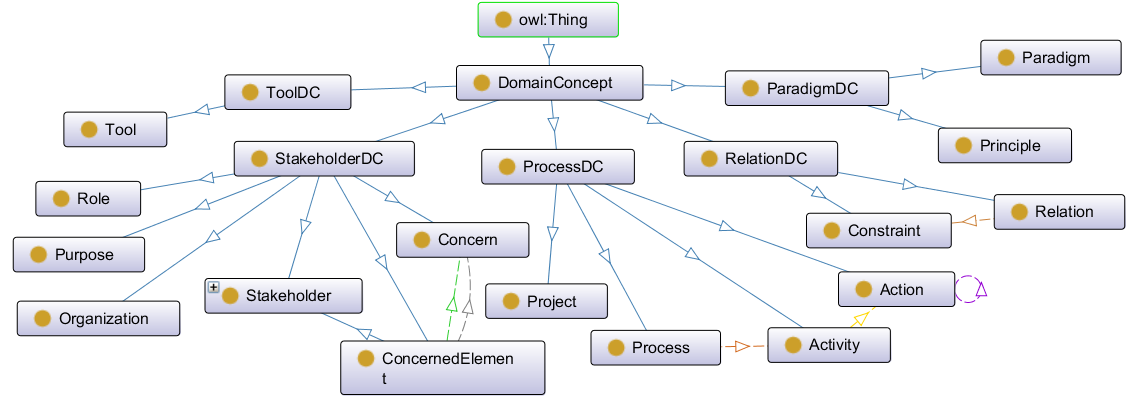
\includegraphics[width=\textwidth]{figures/shared_ontology_overview.png}
\caption{Overview of the shared ontology}
\label{fig:shared_ontology_overview}
\end{figure}

\section{DomainConcept (Domain Concepts)}
\label{sec:shared:classes}

This class groups all domain concepts of the MPM4CPS ontologies. It is further divided into  subclasses for the different sub-domains of the MPM4CPS ontologies. The classes for these sub-domains can be identified from their DC (Domain Concept) suffix. These sub-domain classes allow organizing the ontology into specific domains thus facilitating the navigation across the many concepts of the MPM4CPS ontologies. Note that the sub-domain classes are not disjoint from each other so that a class may belong to several sub-domain concepts.

\subsection{ParadigmDC (Paradigm Domain Concepts)}
\label{subsecDC:ParadigmDC}

This class groups concepts that are related to the \uidxp{paradigm} domain. In this shared ontology, the paradigm domain is introduced in its broad usual sense. These concepts can be refined for the different disciplines such as modeling or programming paradigms.

\subsubsection{Paradigm}
\label{subsubsecC:Paradigm}
\didx{Paradigm}

In the usual sense, a paradigm is a set of concepts, patterns, theories, research methods, postulates, and standards that together constitutes a contribution to a domain.

\textbf{Subclass of}
\begin{itemize}
	\item \textbf{ParadigmDC} (see section \ref{subsecDC:ParadigmDC})
\end{itemize}


\textbf{References}
\begin{itemize}
	
\item \url{https://en.wikipedia.org/wiki/Paradigm}
\end{itemize}




\subsubsection{Principle}
\label{subsubsecC:Principle}
\didx{Principle}

A principle is a law or rule that has to be, or usually is to be followed, or can be desirably followed, or is an inevitable consequence of something, such as the laws observed in nature or the way that a system is constructed. The principles of such a system are understood by its users as the essential characteristics of the system, or reflecting system's designed purpose, and the effective operation or use of which would be impossible if any one of the principles was to be ignored.

\textbf{Subclass of}
\begin{itemize}
	\item \textbf{ParadigmDC} (see section \ref{subsecDC:ParadigmDC})
\end{itemize}


\textbf{References}
\begin{itemize}
	
\item \url{https://en.wikipedia.org/wiki/Principle}
\end{itemize}



\subsection{ProcessDC (Process Domain Concepts)}
\label{subsecDC:ProcessDC}

This class groups concepts that are related to the development \uidxp{process} domain. These concepts were initially inspired from the well-known business process modeling domain. This domain is extremely vast and only a minimal subset from the core business process doamin concepts has been considered and adapted for the MPM4CPS sub-domains (see figure~3.1 of \cite{Weske2019}.

\subsubsection{Activity}
\label{subsubsecC:Activity}
\didx{Activity}

This class represents an activity to be performed during a process. While sometimes the term activity is used for the highest-level business functions. in this framework, an activities represents the finesst grained functions defining the functional perspective of a process.

\textbf{Subclass of}
\begin{itemize}
	\item \textbf{ProcessDC} (see section \ref{subsecDC:ProcessDC})
\end{itemize}


\textbf{References}
\begin{itemize}
	
\item \bibentry{Weske2019 Definition 3.1}
\end{itemize}




\subsubsection{HumanInteractionWorkflow}
\label{subsubsecC:HumanInteractionWorkflow}
\didx{HumanInteractionWorkflow}

A human interaction workflow is a workflow in which humans are actively involved and interact
with information systems.

\textbf{Subclass of}
\begin{itemize}
	\item \textbf{Workflow} (see section \ref{subsubsecC:Workflow})
\end{itemize}


\textbf{References}
\begin{itemize}
	
\item \bibentry{Weske2019 Definition 2.6}
\end{itemize}




\subsubsection{ManualActivity}
\label{subsubsecC:ManualActivity}
\didx{ManualActivity}

A manual activy is an activity that is not supported by information systems.

\textbf{Subclass of}
\begin{itemize}
	\item \textbf{Activity} (see section \ref{subsubsecC:Activity})
\end{itemize}


\textbf{References}
\begin{itemize}
	
\item \bibentry{Weske2019}
\end{itemize}




\subsubsection{Process}
\label{subsubsecC:Process}
\didx{Process}

A process consists of a set of activities that are performed
in coordination in an organizational and technical environment. These
activities jointly realize a business goal. Each business process is enacted by
a single organization, but it may interact with business processes performed
by other organizations.

\textbf{Subclass of}
\begin{itemize}
	\item \textbf{ProcessDC} (see section \ref{subsecDC:ProcessDC})
\end{itemize}


\textbf{References}
\begin{itemize}
	
\item \bibentry{Weske2019 Definition 1.1}
\end{itemize}




\subsubsection{SystemActivity}
\label{subsubsecC:SystemActivity}
\didx{SystemActivity}

A system activy is an activity that is supported by information systems.

\textbf{Subclass of}
\begin{itemize}
	\item \textbf{Activity} (see section \ref{subsubsecC:Activity})
\end{itemize}


\textbf{References}
\begin{itemize}
	
\item \bibentry{Weske2019}
\end{itemize}




\subsubsection{SystemWorkflow}
\label{subsubsecC:SystemWorkflow}
\didx{SystemWorkflow}

A system workflow consists of a workflow in which activities are implemented
by software systems without any user involvement.

\textbf{Subclass of}
\begin{itemize}
	\item \textbf{Workflow} (see section \ref{subsubsecC:Workflow})
\end{itemize}


\textbf{References}
\begin{itemize}
	
\item \bibentry{Weske2019 Definition 2.5}
\end{itemize}




\subsubsection{UserInteractionActivity}
\label{subsubsecC:UserInteractionActivity}
\didx{UserInteractionActivity}

User interaction activities are activities that knowledge workers perform, using information systems.

\textbf{Subclass of}
\begin{itemize}
	\item \textbf{Activity} (see section \ref{subsubsecC:Activity})
\end{itemize}


\textbf{References}
\begin{itemize}
	
\item \bibentry{Weske2019}
\end{itemize}




\subsubsection{Workflow}
\label{subsubsecC:Workflow}
\didx{Workflow}

A workflow is the automation of a business process, in whole
or in part, during which documents, information, or tasks are passed from one
participant to another for action, according to a set of procedural rules.

\textbf{Subclass of}
\begin{itemize}
	\item \textbf{ProcessDC} (see section \ref{subsecDC:ProcessDC})
\end{itemize}


\textbf{References}
\begin{itemize}
	
\item \bibentry{Weske2019 Definition 2.2}
\end{itemize}



\subsection{RelationDC (Relation Domain Concepts)}
\label{subsecDC:RelationDC}

This class groups concepts that are related to the relation domain.

\subsubsection{Constraint}
\label{subsubsecC:Constraint}
\didx{Constraint}

A limitation or a restriction over a relation.

\textbf{Subclass of}
\begin{itemize}
	\item \textbf{RelationDC} (see section \ref{subsecDC:RelationDC})
\end{itemize}






\subsubsection{Relation}
\label{subsubsecC:Relation}
\didx{Relation}

Relation or relations may refer to anything that involves communicating with another person, group, society or country.

\textbf{Subclass of}
\begin{itemize}
	\item \textbf{RelationDC} (see section \ref{subsecDC:RelationDC})
\end{itemize}



\subsection{StakeholderDC (Stakeholder Domain Concepts)}
\label{subsecDC:StakeholderDC}

This class groups concepts that are related to the stakeholder domain.

\subsubsection{Concern}
\label{subsubsecC:Concern}
\didx{Concern}

In computer science, a concern is a particular set of information that has an effect on the code of a computer program. A concern can be as general as the details of database interaction or as specific as performing a primitive calculation, depending on the level of conversation between developers and the program being discussed. IBM uses the term concern space to describe the sectioning of conceptual information.

\textbf{Subclass of}
\begin{itemize}
	\item \textbf{StakeholderDC} (see section \ref{subsecDC:StakeholderDC})
\end{itemize}






\subsubsection{ConcernedElement}
\label{subsubsecC:ConcernedElement}
\didx{ConcernedElement}

\todoAuthors{Provide ``rdfs:comment'' annotation in ontology}

\textbf{Subclass of}
\begin{itemize}
	\item \textbf{StakeholderDC} (see section \ref{subsecDC:StakeholderDC})
	\item \textbf{ConcernedElement} (see section \ref{subsubsecC:ConcernedElement})
\end{itemize}






\subsubsection{Goal}
\label{subsubsecC:Goal}
\didx{Goal}

\todoAuthors{Provide ``rdfs:comment'' annotation in ontology}

\textbf{Subclass of}
\begin{itemize}
	\item \textbf{StakeholderDC} (see section \ref{subsecDC:StakeholderDC})
\end{itemize}






\subsubsection{Organization}
\label{subsubsecC:Organization}
\didx{Organization}

\todoAuthors{Provide ``rdfs:comment'' annotation in ontology}

\textbf{Subclass of}
\begin{itemize}
	\item \textbf{StakeholderDC} (see section \ref{subsecDC:StakeholderDC})
\end{itemize}






\subsubsection{Purpose}
\label{subsubsecC:Purpose}
\didx{Purpose}

The object for which something exists

\textbf{Subclass of}
\begin{itemize}
	\item \textbf{StakeholderDC} (see section \ref{subsecDC:StakeholderDC})
\end{itemize}






\subsubsection{Role}
\label{subsubsecC:Role}
\didx{Role}

A role (also role or social role) is a set of connected behaviours, rights, obligations, beliefs, and norms as conceptualized by people in a social situation. It is an expected or free or continuously changing behaviour and may have a given individual social status or social position. It is vital to both functionalist and interactionist understandings of society.

\textbf{Subclass of}
\begin{itemize}
	\item \textbf{StakeholderDC} (see section \ref{subsecDC:StakeholderDC})
\end{itemize}






\subsubsection{Stakeholder}
\label{subsubsecC:Stakeholder}
\didx{Stakeholder}

A stakeholder or stakeholders, as defined in its first usage in a 1963 internal memorandum at the Stanford Research Institute, are "those groups without whose support the organization would cease to exist." The theory was later developed and championed by R. Edward Freeman in the 1980s. Since then it has gained wide acceptance in business practice and in theorizing relating to strategic management, corporate governance, business purpose and corporate social responsibility (CSR). A corporate stakeholder can affect or be affected by the actions of a business as a whole.

\textbf{Subclass of}
\begin{itemize}
	\item \textbf{ConcernedElement} (see section \ref{subsubsecC:ConcernedElement})
	\item \textbf{StakeholderDC} (see section \ref{subsecDC:StakeholderDC})
\end{itemize}






\subsubsection{ToolProvider}
\label{subsubsecC:ToolProvider}
\didx{ToolProvider}

Who provides the product and gives the licenses (e.g. company, university, group, ..)

\textbf{Subclass of}
\begin{itemize}
	\item \textbf{Stakeholder} (see section \ref{subsubsecC:Stakeholder})
\end{itemize}



\subsection{ToolDC (Tool Domain Concepts)}
\label{subsecDC:ToolDC}

This class groups concepts that are related to the tool domain.

\subsubsection{Tool}
\label{subsubsecC:Tool}
\didx{Tool}

Set of different tools that are used during system development.

\textbf{Subclass of}
\begin{itemize}
	\item \textbf{ToolDC} (see section \ref{subsecDC:ToolDC})
\end{itemize}

\section{Properties}
\label{sec:shared:properties}


\subsection{hasActivities}
\label{subsecP:hasActivities}
Represents the activities that a process may use through its workflows.
Subproperty of:
None


Domains:
\begin{itemize}
	\item \textbf{Process} (see section \ref{subsubsecC:Process})
\end{itemize}


Ranges:
\begin{itemize}
	\item \textbf{Activity} (see section \ref{subsubsecC:Activity})
\end{itemize}




\subsection{hasConcerns}
\label{subsecP:hasConcerns}
A concern of stakeholder.
Subproperty of:
None


Domains:
\begin{itemize}
	\item \textbf{ConcernedElement} (see section \ref{subsubsecC:ConcernedElement})
\end{itemize}


Ranges:
\begin{itemize}
	\item \textbf{Concern} (see section \ref{subsubsecC:Concern})
\end{itemize}




\subsection{hasConstraint}
\label{subsecP:hasConstraint}
A constraint applied on relation.
Subproperty of:
None


Domains:
\begin{itemize}
	\item \textbf{Relation} (see section \ref{subsubsecC:Relation})
\end{itemize}


Ranges:
\begin{itemize}
	\item \textbf{Constraint} (see section \ref{subsubsecC:Constraint})
\end{itemize}




\subsection{hasEnactedActivities}
\label{subsecP:hasEnactedActivities}
Represents the activities that a workflow enacts.
Subproperty of:
None


Domains:
\begin{itemize}
	\item \textbf{Workflow} (see section \ref{subsubsecC:Workflow})
\end{itemize}


Ranges:
\begin{itemize}
	\item \textbf{Activity} (see section \ref{subsubsecC:Activity})
\end{itemize}




\subsection{hasEvolvedTo}
\label{subsecP:hasEvolvedTo}
An updated version of an element. (e.g.Tool evolved to another)
Subproperty of:
None


Domains:
None


Ranges:
None




\subsection{hasNext}
\label{subsecP:hasNext}
\todoAuthors{Provide ``rdfs:comment'' annotation in ontology}
Subproperty of:
None


Domains:
None


Ranges:
None




\subsection{hasProvider}
\label{subsecP:hasProvider}
The company/university which the tool is developed by.
Subproperty of:
None


Domains:
None


Ranges:
None




\subsection{hasRole}
\label{subsecP:hasRole}
A role of stakeholder
Subproperty of:
None


Domains:
\begin{itemize}
	\item \textbf{Stakeholder} (see section \ref{subsubsecC:Stakeholder})
\end{itemize}


Ranges:
\begin{itemize}
	\item exactly 1 \textbf{Role} (see section \ref{subsubsecC:Role})
\end{itemize}




\subsection{hasSystemActivities}
\label{subsecP:hasSystemActivities}
\todoAuthors{Provide ``rdfs:comment'' annotation in ontology}
Subproperty of:
\begin{itemize}
	\item \textbf{hasEnactedActivities} (see section \ref{subsecP:hasEnactedActivities})
\end{itemize}


Domains:
None


Ranges:
\begin{itemize}
	\item \textbf{SystemActivity} (see section \ref{subsubsecC:SystemActivity})
\end{itemize}




\subsection{hasUserInteractionActivities}
\label{subsecP:hasUserInteractionActivities}
\todoAuthors{Provide ``rdfs:comment'' annotation in ontology}
Subproperty of:
\begin{itemize}
	\item \textbf{hasEnactedActivities} (see section \ref{subsecP:hasEnactedActivities})
\end{itemize}


Domains:
None


Ranges:
\begin{itemize}
	\item \textbf{UserInteractionActivity} (see section \ref{subsubsecC:UserInteractionActivity})
\end{itemize}




\subsection{hasWorkflows}
\label{subsecP:hasWorkflows}
\todoAuthors{Provide ``rdfs:comment'' annotation in ontology}
Subproperty of:
None


Domains:
\begin{itemize}
	\item \textbf{Process} (see section \ref{subsubsecC:Process})
\end{itemize}


Ranges:
\begin{itemize}
	\item \textbf{Workflow} (see section \ref{subsubsecC:Workflow})
\end{itemize}




\subsection{isAppliedTo}
\label{subsecP:isAppliedTo}
A constraint is applied to a some element. (e.g. relation)
Subproperty of:
None


Domains:
\begin{itemize}
	\item \textbf{Constraint} (see section \ref{subsubsecC:Constraint})
\end{itemize}


Ranges:
None




